\section{Introduction} 
Nowadays, there exists huge amounts of spatiotemporal data in various fields of science.
% such as agriculture, transportation and social science.
Analysis of such data is interesting as it is grounded
on reality: each record represents a specific location and time. Moreover, understanding patterns and trends provides analysis insights leading to improved user planning and decision making. Some instance applications of spatiotemporal data are smart city management, disaster management and autonomous transport.
% \cite{RoddickEHPS04,Telang:2012}.

\begin{figure}[t]
  \centering
  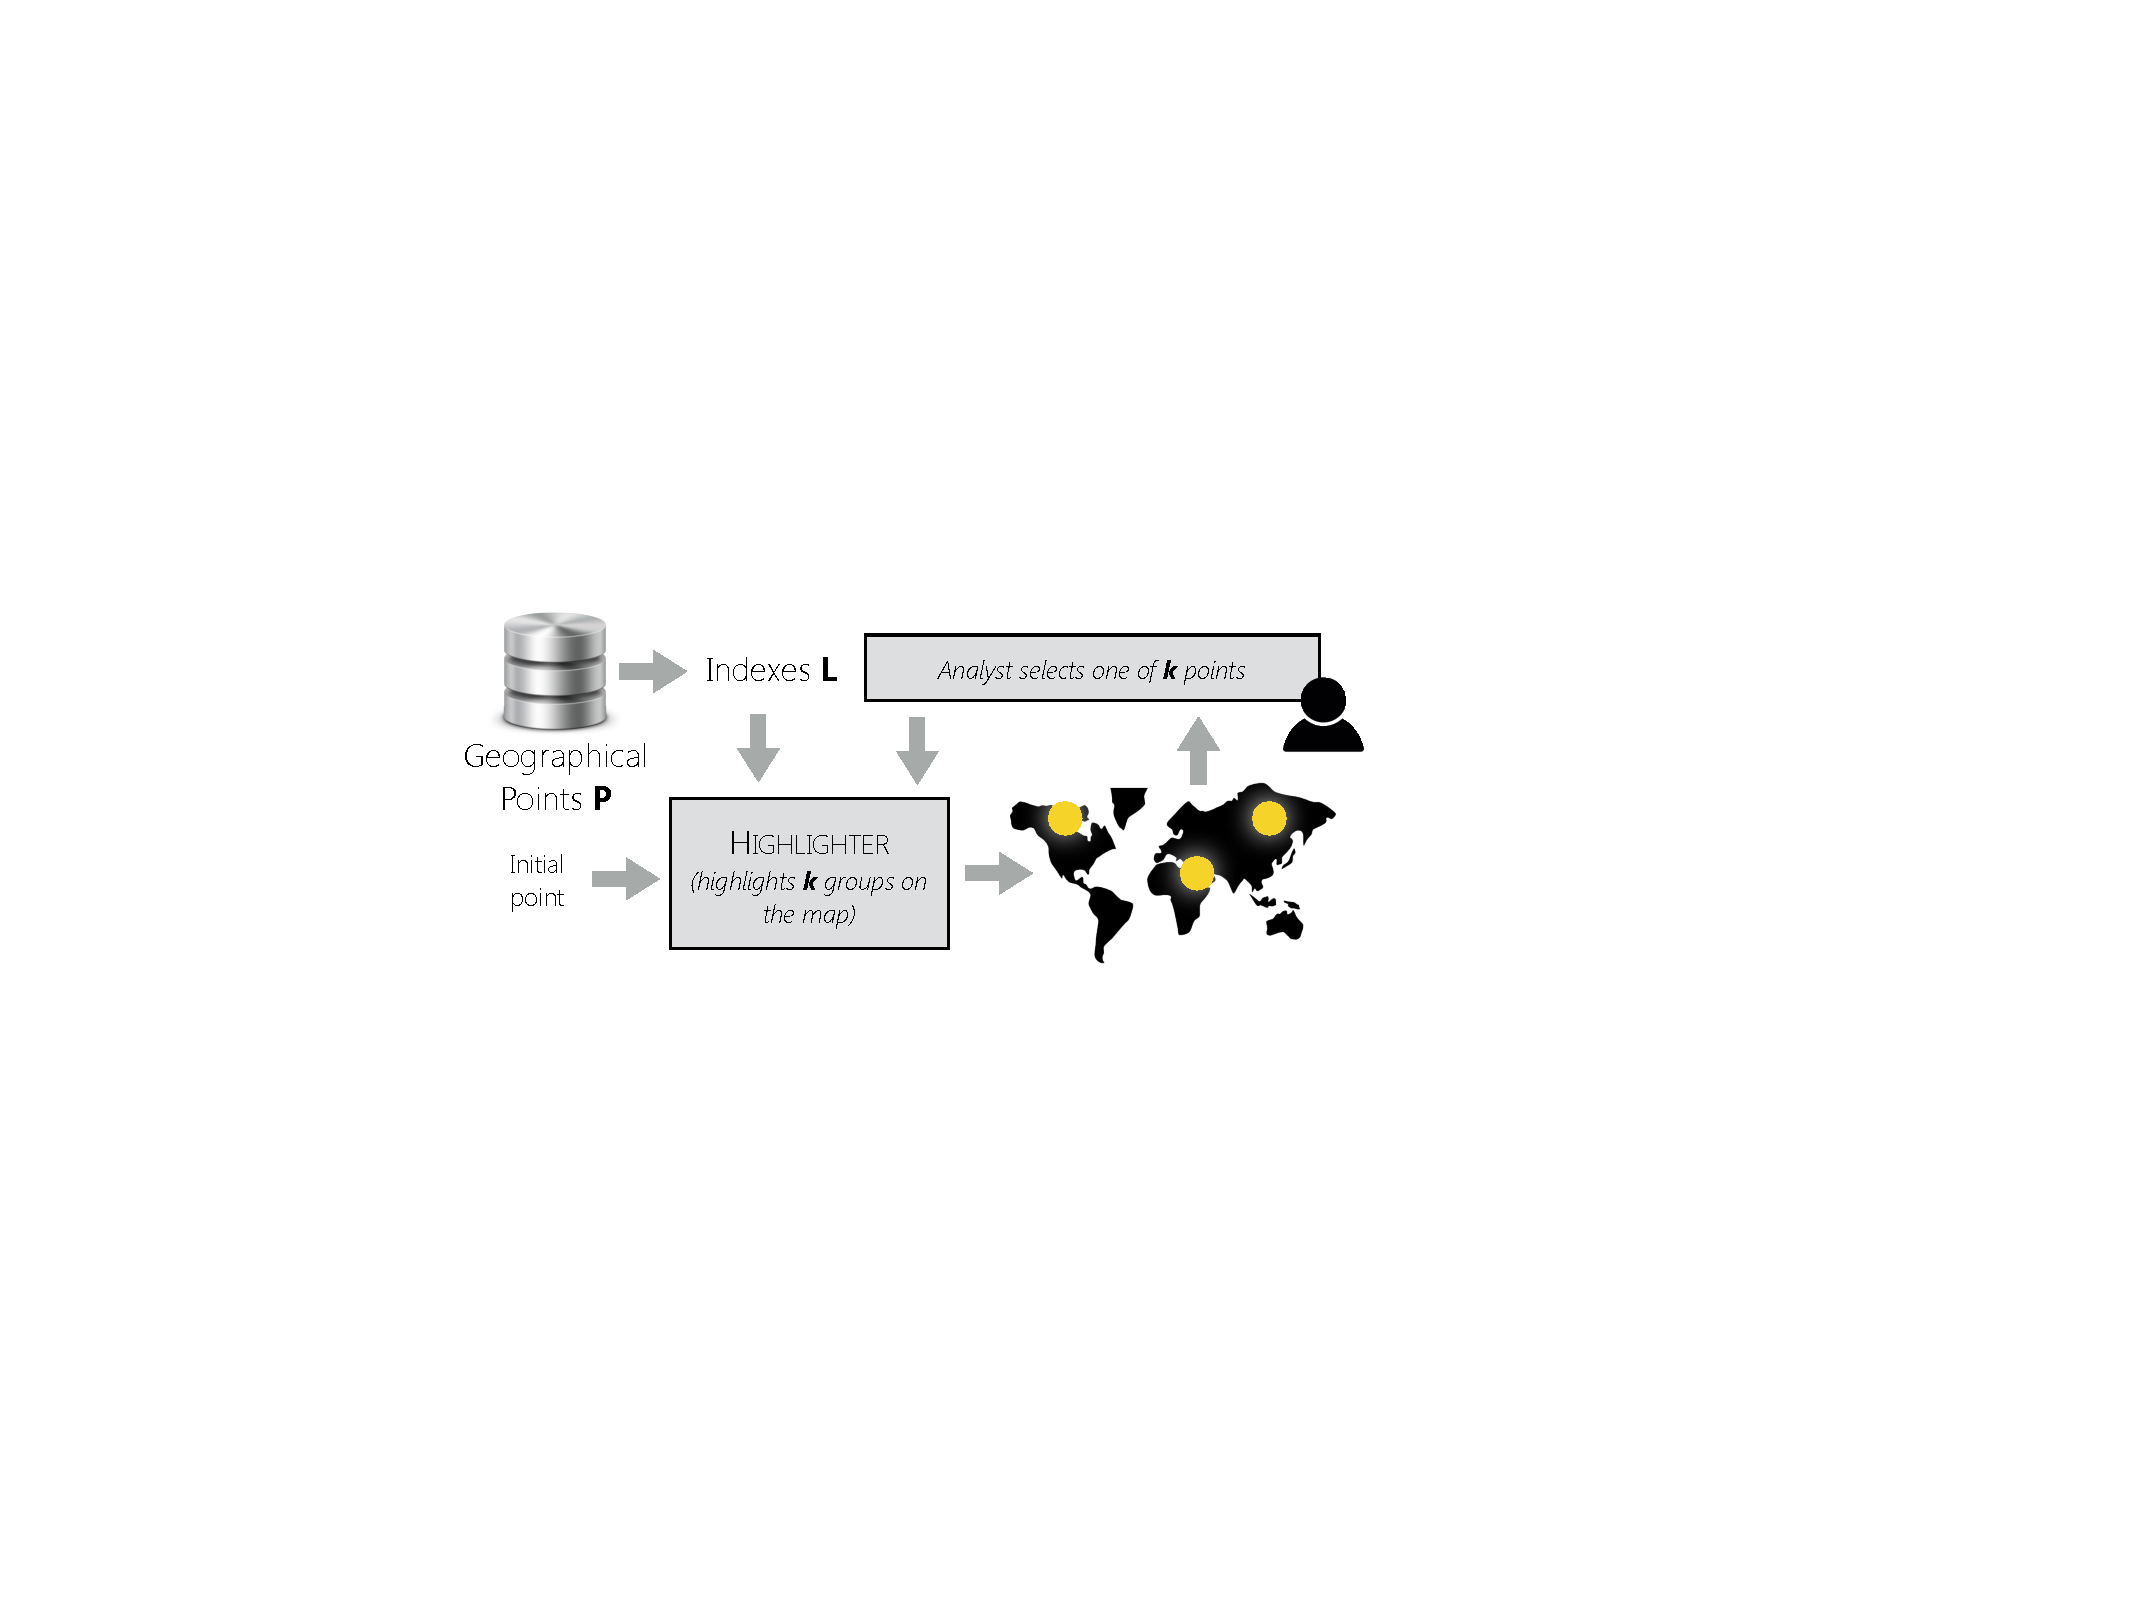
\includegraphics[width=\columnwidth]{figs/framework}
\caption{\framework\ Framework}
\label{fig:framework}
\vspace{-10pt}
\end{figure}

Traditionally, an exploratory analysis scenario on spatiotemporal data is described as follows: the analyst visualizes the data using an off-the-shelf product (e.g., Tableau\footnote{\it http://www.tableau.com},
% Exhibit\footnote{\it http://www.simile-widgets.org/exhibit/},
Spotfire\footnote{\it http://spotfire.tibco.com}). Then she looks at different parts of data for interesting patterns and trends. With the growing size of spatiotemporal datasets, this classical approach is not practical anymore: geographical points are scattered everywhere and the analyst cannot effectively observe insights.

To overcome this challenge, visualization environments offer a plethora of operations to manipulate data (filter, aggregate, etc.). In practice, this duplicates the problem: the analyst is left alone in a huge space of data and operations. 
In an exploratory context,
%Considering the exploratory context as a non-idempotent process\footnote{\it We call an interactive step as ``idempotent'' if it always follows the exact same steps.},
the principled challenge for the analyst is {\em ``what to see next''} during the analysis process. A {\em guidance mechanism} is necessary to point out potential future directions of analysis.

Given a geographical point of interest, the question is then how to recommend other points to be considered in future analysis steps in form of guidance. In this paper, we focus on one specific guidance approach, i.e., highlighting $k$-best points given a point of interest. Those $k$ points should have high quality. Quality is formulated as optimization of two dimensions: {\em relevance} and {\em diversity}. Optimizing relevance ensures that recommended points are in-line with what the analyst has already liked. Optimizing diversity results points which are as different as possible from each other and unveil different aspects of analysis. Example \ref{ex:flight} illustrates a common case in practice.

\begin{example}
\label{ex:flight}
Tiffany is a data scientist and is tasked to design a {\em chain marketing} strategy for a Peking Duck product whose headquarters is in New York. She already knows that the product has success in the local area. So she analyzes Yelp data\footnote{\it https://www.yelp.com/} (i.e., restaurant check-ins) to find out what other locations exhibit similar eating profiles as New York. She asks for $k$ geographical points which have relevant eating profile to New York and are the most diverse. Given $k=3$, Tiffany receives points from San Fransisco, Washington DC and Marlton, NJ. She selects Marlton due to its proximity to reduce transportation costs. Then she asks for other 3 best points for Marlton. She can then make the city-to-city chain marketing strategy.
\end{example}

In this paper, we address the problem of guidance. Despite the great progress on spatiotemporal data analysis in recent years, we point out following challenges for guidance:
$i.$ {\em Genericness.} Considering the heterogeneous nature of spatiotemporal datasets, it is challenging to come up with a generic guidance approach which is independent of data type and distribution.
$ii.$ {\em Size}. The gigantic size of spatiotemporal datasets hinders its effective discovery. 
% The guidance approach should be able to provide a limited set of recommendations to overcome information overload.
$iii.$ {\em Efficiency.} Guidance should be done efficiently in consecutive steps, so that the train of the analyst's thoughts won't break. Despite progress in efficient spatiotemporal processing \cite{yu2015geospark}, sub-second interactivity is still missing.

% In terms of efficiency, {\sc GeoSpark} \cite{yu2015geospark} and {\sc SpatialHadoop} \cite{DBLP:conf/icde/EldawyM15} are two promising computing systems for efficient processing large-scale spatiotemporal data. Those systems can exploited as the backbone of \framework\ once large-scale data needs to be analyzed.

% \vspace{5pt}
% \noindent {\bf Related Work.}
There exist few instances of information-highlighting methods \cite{Liang2010,Robinson2011,wongsuphasawat2016voyager,willett2007scented}. However all these methods are {\em objective} and do not apply to the context of spatiotemporal guidance where user feedback is involved.  In terms of recommendation, few approaches focus on spatial dimension
% \cite{Levandoski:2012,Magdy2014,HendawiKRBTA15a,Bao2015,Magdy:2014}
\cite{Bao2015,Levandoski:2012}
while the context and result diversification are missing.
% In this paper, we addressed the problem of highlighting geographical points to
% guide analysts in consecutives steps. To the best of our knowledge, this is the
% first work which formulates the geo-highlighting problem for recommending on
% maps. However, our problem relates to a number of others as follows.     

% Visual Highlighting. There has been efforts to highlight some pieces of
% information in the huge heterogeneous data space so that the analyst can focus
% on important aspects \cite{}. Visual
% Story Construction is another domain of work \cite{} which
% consecutive analysis steps are created automatically. However, all such highlighting methods are objective and does not consider analyst
% interest. In GeoHiglight, we provide a simple yet effective feedback model which
% can feed the recommendation algorithm to produce relevant results to current
% investigations.        

% Some other works have exploited highlighting as a technique to synchronize
% coordinated views [CITE CROSSFILTER] or simplify complicated dataset
% visualizations \cite{Robinson2011,Alper:2011}. Also in \cite{Philipsen}
% different highlighting methods are compared in terms of efficiency and usefulness. Such methods are complementary to ours.     

% Spatiotemporal Interactive Analysis and Visualization. Being an interactive
% system, it should be efficient and capture user feedback and adapt the utility
% function. In terms of efficiency, SpatialHadoop \cite{} and GeoSpark \cite{}
% extend Hadoop and Spark ecosystems respectively to boost geographical
% computations and visualizations. Such systems can be exploited as the backbone
% of GeoHighlight once large-scale data needs to be analyzed.      

% In terms of feedback, many off-the-shelf products such as Tableau \cite{} and
% RapidMiner \cite{} are designed to visualize different kinds of datasets including
% spatiotemporal ones. However, ``recommendation'' is the missing component in
% most of such tools: providing a full package of operations and actions, the analyst
% may know what to do next. In such system, analysis is usually considered as a
% one-shot scenario, once in reality it happens in consecutive steps following
% user feedback.        

% Recommendation. There exist a huge body of work in recommendation
% \cite{Adomavicius:2005} for various domains and datasets. However, spatial
% dimension is still untouched and has not received a lot of attention. In
% \cite{ChirigatiDDF16} a prediction algorithm for urban data is introduced which operates offline. In
% \cite{Levandoski:2012,Magdy2014,HendawiKRBTA15a,Bao2015,Magdy:2014},
% recommendation and visualization tools are introduced in specific domains.
% However, most the such algorithms are not context-aware (based on user choices)
% and does not consider diversity as a global metric.    


% \vspace{5pt}
In this paper, we propose a generic interactive analysis approach for guiding analysts towards potential interesting points. The analyst considers the guidance and picks a direction for the next analysis iteration. 

% prune this
% \vspace{5pt}
% \noindent {\bf Outline.} in Section \ref{sec:data-model}, we present our data model. Then in Section \ref{sec:pb}, we formally define our problem. Section \ref{sec:algo} describes our solution for the guidance problem. We show a realistic application of our solution in Section \ref{sec:scenarios}. We present an extensive set of experiments in Section \ref{sec:exp}. A summary of related work is discussed in Section \ref{sec:rel}. Finally we conclude in Section \ref{sec:conc}.